\documentclass[lettersize,journal]{IEEEtran}
\usepackage{amsmath,amsfonts}
\usepackage{algorithmic}
\usepackage{array}
\usepackage[caption=false,font=normalsize,labelfont=sf,textfont=sf]{subfig}
\usepackage{textcomp}
\usepackage{stfloats}
\usepackage{url}
\usepackage{verbatim}
\usepackage{graphicx}
\usepackage{multirow}
\usepackage[portuguese]{babel}

\hyphenation{op-tical net-works semi-conduc-tor IEEE-Xplore}
\def\BibTeX{{\rm B\kern-.05em{\sc i\kern-.025em b}\kern-.08em
    T\kern-.1667em\lower.7ex\hbox{E}\kern-.125emX}}
\usepackage{balance}
\begin{document}
\title{Relatório de Treinamento \\ Machine Learning – LBP + KNN}
\author{Barbara Reis dos Santos
\thanks{Este trabalho foi desenvolvido no Departamento de Informática da Universidade Federal do Paraná (UFPR), sob a orientação do professor Paulo Ricardo Lisboa de Almeida.}}
\maketitle

\begin{abstract}
Este relatório descreve o processo de treinamento de um modelo de Aprendizado de Máquina utilizando os métodos LBP (Padrões Binários Locais) e KNN (K-Vizinhos Mais Próximos). O objetivo deste trabalho é explorar conceitos básicos de Aprendizado de Máquina clássico, incluindo extração de características e criação de classificadores usando aprendizado supervisionado.
\end{abstract}

\begin{IEEEkeywords}
Aprendizado de Máquina, LBP, KNN, classificação, extração de características, histograma, detecção de vagas de estacionamento.
\end{IEEEkeywords}

\section{Introdução}

Os sistemas de detecção de vagas em estacionamentos externos têm despertado grande interesse na última década devido às suas diversas aplicações práticas. Recentemente, foi apresentado um novo conjunto de dados de estacionamento composto por 695.899 imagens capturadas de dois estacionamentos, cada um com três visualizações de câmeras distintas \cite{almeida2015pklot}. Nesse conjunto de dados, foi avaliado o desempenho de dois descritores texturais, os Padrões Binários Locais (LBP) e a Fase Local de Quantização (LPQ), para a detecção de vagas de estacionamento. Este relatório descreve o processo de treinamento de um modelo de Aprendizado de Máquina que utiliza o descritor textural LBP e o método KNN para classificar vagas de estacionamento como vazias ou ocupadas, a partir do conjunto de dados mencionado. O objetivo é explorar conceitos básicos de Aprendizado de Máquina clássico na prática, utilizando um problema real, incluindo extração de características e aprendizado supervisionado, para alcançar uma detecção precisa da ocupação de estacionamentos.

\section{Revisão Bibliográfica}
O método LBP (Local Binary Patterns) é uma técnica amplamente utilizada em processamento de imagens para a extração de características locais. Proposto por Ojala et al. em 1996 \cite{ojala2002multiresolution}, o LBP representa cada pixel de uma imagem por um valor binário, comparando-o com seus vizinhos e codificando a relação de intensidade entre eles. Esses padrões binários locais são então utilizados como características para descrever texturas e formas em imagens.

Por outro lado, o algoritmo KNN (K-Nearest Neighbors) é um método simples de classificação que se baseia na proximidade entre os pontos no espaço de características. Ao classificar um novo exemplo, o KNN identifica os k vizinhos mais próximos do ponto de interesse e atribui a ele a classe mais comum entre esses vizinhos.

\section{Metodologia}

Para o processo de treinamento, foram utilizados os seguintes passos:

1) Obtenção dos dados: Os dados utilizados foram extraídos da base PKLot, disponível em \url{https://web.inf.ufpr.br/vri/databases/parking-lot-database/}.

2) Extração de características: Para cada imagem da base de dados, foram extraídas as características LBP (Local Binary Patterns) considerando uma vizinhança de tamanho oito. As características LBP foram então calculadas para cada pixel da imagem.

3) Cálculo do histograma: Para cada imagem, foi calculado o histograma das características LBP, representando a distribuição das características na imagem.

4) Geração dos vetores de características: Utilizando os histogramas, foi criado um arquivo CSV que representa o conjunto de dados. Cada linha do arquivo corresponde a uma imagem, e cada coluna representa uma característica extraída usando o método LBP. Além disso, ao final de cada linha, há uma indicação da classe da imagem, onde a classe é 1 se a imagem representa uma vaga ocupada ou 0 se a imagem representa uma vaga vazia.

5) Divisão dos dados: O conjunto de dados foi dividido em conjuntos de treinamento e teste, sendo 70\% dos dados para treinamento e 30\% para teste. 

6) Normalização dos dados: Os histogramas LBP foram normalizados utilizando a técnica min-max. A instância de teste foi normalizada utilizando os mesmos parâmetros de normalização que a instância de treinamento.

7) Treinamento do modelo KNN: Um classificador KNN foi treinado com k=3, utilizando os dados de treinamento normalizados.

8) Avaliação do modelo: O modelo KNN treinado foi avaliado utilizando o conjunto de dados de teste, calculando-se a acurácia e a matriz confusão do modelo.


\section{Discussão e Resultados}

\subsection{Análise da Divisão dos Dados}

A divisão dos dados em conjuntos de treinamento e teste foi realizada de forma aleatória, garantindo que a proporção entre as classes fosse mantida em ambos os conjuntos. Essa abordagem aleatória é fundamental para evitar vieses nos conjuntos de dados de treinamento e teste.A divisão aleatória foi feita com o uso do parâmetro \texttt{random\_state=5}, que fixa a semente do gerador de números aleatórios para garantir a reprodutibilidade dos resultados. Assim, ao manter a aleatoriedade controlada, podemos confiar na generalização do modelo para dados futuros sem introduzir viés na avaliação do seu desempenho.

\subsection{Escolha do Valor de K para o KNN}

O valor de K escolhido foi K=3, selecionado com base na simplicidade do problema. Com apenas duas classes, um valor moderadamente baixo de k pode capturar padrões relevantes nos dados sem ser excessivamente sensível ao ruído. Um valor muito alto de k poderia suavizar demais as fronteiras de decisão, tornando o modelo menos sensível às nuances nos dados.

\subsection{Interpretação da Matriz de Confusão}

A matriz de confusão fornece informações mais detalhadas sobre o desempenho do modelo do que a simples acurácia. Algumas conclusões importantes que podem ser extraídas da matriz de confusão e que não seriam evidentes apenas olhando para a acurácia são: Desequilíbrio de classes, taxa de Falsos Positivos e Falsos Negativos, análise de Erros Específicos, entre outras.


O modelo de classificação foi treinado e testado utilizando uma amostra reduzida do conjunto de dados devido a limitação de memória da máquina utilizada. Apesar da redução da amostra, os resultados obtidos foram satisfatórios, com uma acurácia de 89.41\% na classificação das imagens. A matriz de confusão gerada a partir do conjunto de dados utilizando 5\% do original é mostrada na Tabela \ref{tab:confusion_matrix}.

\begin{table}[htbp]
    \centering
    \begin{tabular}{cc|c|c|}
        \cline{3-4}
        & & \multicolumn{2}{c|}{\textbf{Valores Previstos}} \\ \cline{3-4} 
        & & \textbf{Empty} & \textbf{Occupied} \\ \hline
        \multicolumn{1}{|c|}{\multirow{2}{*}{\textbf{Valores Reais}}} & \textbf{Empty} & 5172 & 155 \\ \cline{2-4} 
        \multicolumn{1}{|c|}{} & \textbf{Occupied} & 950 & 4161 \\ \hline
    \end{tabular}\vspace{5pt}
    \caption{Matriz de confusão.}
    \label{tab:confusion_matrix}
\end{table}

\subsection{LBP e Histograma}

\begin{figure}[h]
    \centering
    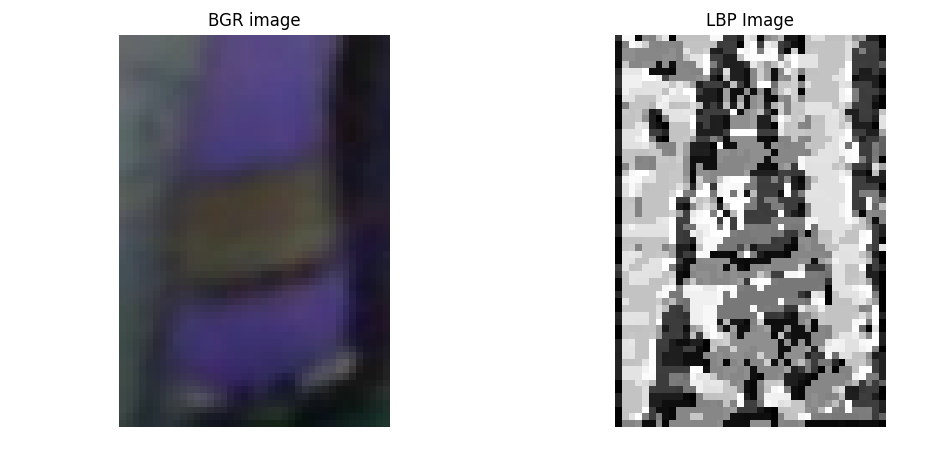
\includegraphics[width=0.4\textwidth]{LBP_Image.png}
    \caption{Imagem Original e LBP}
\end{figure}

Na figura 1, à esquerda, mostra a imagem original de uma das vagas de estacionamento e, à direita, a imagem após a aplicação do LBP.

\begin{figure}[h]
    \centering
    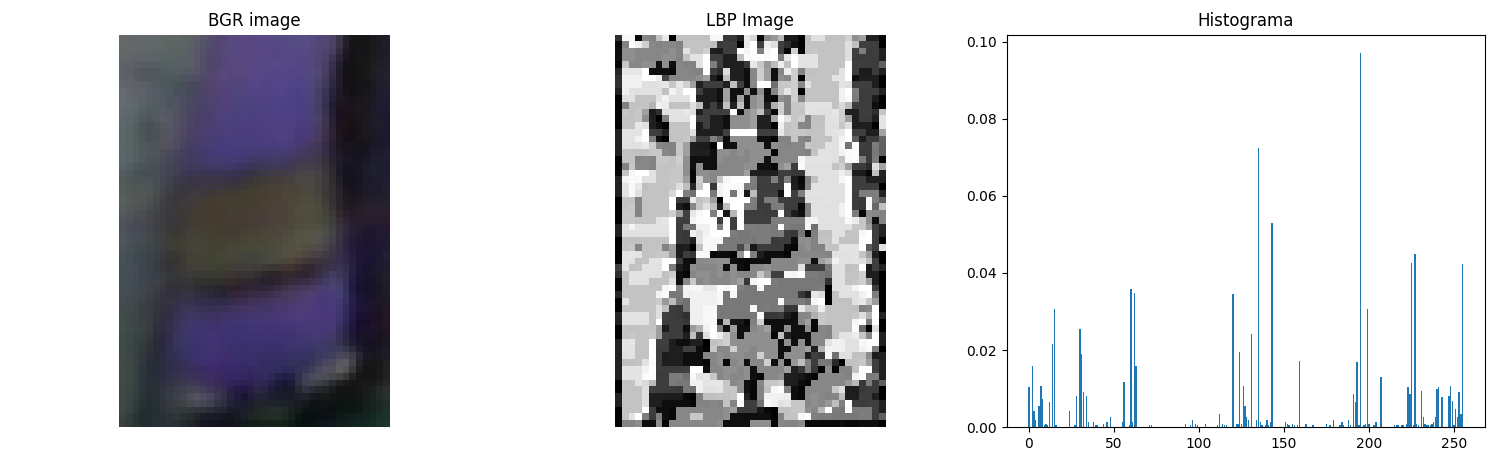
\includegraphics[width=0.4\textwidth]{histogram.png}
    \caption{Histograma LBP}
\end{figure}

O histograma exibido na figura 2 representa as características extraídas da imagem após a aplicação do algoritmo LBP. Ele é composto por 256 barras, uma para cada possível valor de intensidade de pixel (de 0 a 255) na imagem LBP.

Na horizontal, temos os valores de intensidade, que variam de 0 a 255, representando as características únicas da imagem resultantes da transformação LBP. Cada barra vertical indica a frequência com que cada valor de intensidade aparece na imagem, fornecendo assim uma representação visual da distribuição dessas características.


\section{Conclusão}
Em resumo, os resultados deste estudo destacam a eficácia da combinação do método LBP com o classificador KNN para a classificação de vagas de estacionamento. No entanto, para futuras melhorias, é fundamental aprimorar a otimização de memória, além de explorar outras técnicas de extração de características, classificadores e algoritmos mais avançados de aprendizado de máquina. Esses passos podem contribuir significativamente para aumentar a precisão e eficiência do sistema de detecção de vagas de estacionamento.

\begin{thebibliography}{1}

\bibitem{ojala2002multiresolution}
Ojala, T., Pietikainen, M., \& Maenpaa, T. (2002). Multiresolution gray-scale and rotation invariant texture classification with local binary patterns. \textit{IEEE Transactions on Pattern Analysis and Machine Intelligence}, 24(7), 971-987.

\bibitem{medium}
Featurepreneur. (n.d.). Understanding the concept of channels in an image. \textit{Medium}. Recuperado de \url{https://medium.com/featurepreneur/understanding-the-concept-of-channels-in-an-image-6d59d4dafaa9}

\bibitem{brasilai}
Brasil AI. (n.d.). KNN - K Nearest Neighbors. \textit{Medium}. Recuperado de \url{https://medium.com/brasil-ai/knn-k-nearest-neighbors-1-e140c82e9c4e}

\bibitem{almeida2015pklot}
P. R. De Almeida, L. S. Oliveira, A. S. Britto Jr, E. J. Silva Jr, and A. L. Koerich, “Pklot–a robust dataset for parking lot classification,” \textit{Expert Systems with Applications}, vol. 42, no. 11, pp. 4937–4949, 2015. Recuperado de \url{https://web.inf.ufpr.br/vri/databases/parking-lot-database/}

\end{thebibliography}

\end{document}
